% \documentclass[handout]{beamer}
\documentclass[presentation]{beamer}

\usepackage[utf8]{inputenc}
\usepackage[UKenglish]{babel}
\usepackage{booktabs}
\usepackage{caption}
\usepackage{subcaption}
\usepackage{graphicx}
\usepackage{amsmath}
\usepackage{amsfonts}
\usepackage{amssymb}
\usepackage{epstopdf}
\usepackage{hyperref}

% complying UK date format, i.e. 1 January 2001
\usepackage{datetime}
\let\dateUKenglish\relax
\newdateformat{dateUKenglish}{\THEDAY~\monthname[\THEMONTH] \THEYEAR}

\usecolortheme{Imperial}
% -----------------------------------------------------------------------------
%Information to be included in the title page:
\title{Addressing Security in Control Systems}
\subtitle{Overview and Current Directions}
\author{Angelo Barboni}

\date{17 September 2019}

\begin{document}
 
\begin{frame}[noframenumbering,plain]
\titlepage
\end{frame}

\begin{frame}[noframenumbering,plain]{Outline}
    \tableofcontents
\end{frame}


\section{Introduction}

\begin{frame}
	\frametitle{Security goals}

	Security (of information) can be attained if these properties are satisfied:
	\vfill
	\begin{description}
		\item[Confidentiality] Concealment or protection of sensitive information
		\item[Integrity] Trustworthiness and authenticity of data or resources 
		\item[Availability] Reliable and timely access to desired information 
	\end{description}
	\vfill
	\null
\end{frame}

\begin{frame}
	\frametitle{Motivation}
	\begin{center}
		Cyber-Physical Systems (CPS) $=$ \\ (complex, connected) software $+$ hardware
	\end{center}
	\vspace{-1ex}
	\begin{columns}
		\begin{column}{0.35\textwidth}
			Software is vulnerable: it \emph{will} be exploited. 

			\vspace{3ex}
			Security has be thought of in a system way.
		\end{column}
		\begin{column}{0.64\textwidth}
			\begin{figure}
				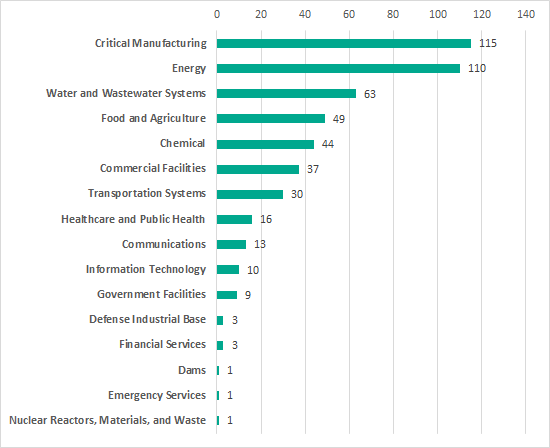
\includegraphics[scale=0.44]{fig/vuln-report-ics-cert.png}
				\caption*{\footnotesize Vulnerabilities in 2018 by sector [\href{https://ics-cert.us-cert.gov/}{\color{blue}{\underline{US ICS-CERT}}}]}
			\end{figure}
		\end{column}
	\end{columns}
\end{frame}

\begin{frame}
	\frametitle{A (possibly incomplete) series of unfortunate events}
	\setbeamertemplate{description item}[align left]
	\begin{description}
		\item[2000] Maroochy Shire incident (Australia)
		\item[2007] Aurora generator test (USA)
		\item[2009-2010] Stuxnet worm (Iran)
		\item[2014] Steel mill (Germany)
		\item[2015] Blackout (Ukraine)
		\item[2017] TRITON malware, oil spill (Saudi Arabia)
		\item[2019] Power grid DoS (USA)  
	\end{description}
\end{frame}

\begin{frame}
	\frametitle{Disclaimer}

	The topic of security encompasses many fields, from dedicated software security (PLCs, SCADA systems), to application specific cases (power networks, mobile networks, multiagent systems, etc.).

	\vfill
	We follow a generic system approach.
\end{frame}

\AtBeginSection[]
{
  \begin{frame}[noframenumbering,plain]{Outline}
    \tableofcontents[currentsection,hideallsubsections]
  \end{frame}
}

\section{Adversarial model}

\section{Taxonomy}

\section{Distributed Systems}

\section{What's next?}

 
\end{document}